\documentclass[12pt]{beamer}

\usepackage{color}
\usepackage[T2A]{fontenc}

\usepackage[absolute,overlay]{textpos}
\usepackage{setspace}
\usepackage[export]{adjustbox}
\usepackage{wrapfig}
\usepackage{csquotes}

\defbeamertemplate{footline}{centered page number}
{%
  \hspace*{\fill}%
  \usebeamercolor[fg]{page number in head/foot}%
  \usebeamerfont{page number in head/foot}%
  \insertpagenumber\,/\,\insertpresentationendpage%
  \hspace*{\fill}\vskip2pt%
}
\setbeamertemplate{footline}[centered page number]
%\mode<presentation>{
%\usetheme{Rochester}
%}
\newcommand{\backupbegin}{
   \newcounter{framenumberappendix}
   \setcounter{framenumberappendix}{\value{framenumber}}
}
\newcommand{\backupend}{
   \addtocounter{framenumberappendix}{-\value{framenumber}}
   \addtocounter{framenumber}{\value{framenumberappendix}} 
}
\mode<presentation>{
  \usetheme{AnnArbor}
}
\makeatletter
\setbeamertemplate{footline}
{
  \leavevmode%
  \hbox{%
  \begin{beamercolorbox}[wd=.333333\paperwidth,ht=2.25ex,dp=1ex,center]{author in head/foot}%
    \usebeamerfont{author in head/foot}\insertshortauthor%~~\beamer@ifempty{\insertshortinstitute}{}{(\insertshortinstitute)}
  \end{beamercolorbox}%
  \begin{beamercolorbox}[wd=.333333\paperwidth,ht=2.25ex,dp=1ex,center]{title in head/foot}%
    \usebeamerfont{title in head/foot}\insertshorttitle
  \end{beamercolorbox}%
  \begin{beamercolorbox}[wd=.333333\paperwidth,ht=2.25ex,dp=1ex,right]{date in head/foot}%
    \usebeamerfont{date in head/foot}\insertshortdate{}\hspace*{2em}
    \insertframenumber{} / \inserttotalframenumber\hspace*{2ex} 
  \end{beamercolorbox}}%
  \vskip0pt%
}
\makeatother

\setbeamertemplate{navigation symbols}{}

\setbeamercolor{frametitle}{fg=black,bg=white}
\setbeamercolor{title}{fg=black,bg=yellow!85!orange}

\beamersetuncovermixins{\opaqueness<1>{25}}{\opaqueness<2->{15}}


\begin{document}

\title{Gaussian processes introduction}
\author{Victor Kocheganov}
\date{\today} 

\begin{frame}
\titlepage
\end{frame}

\begin{frame}{Problem statement}
\begin{figure}
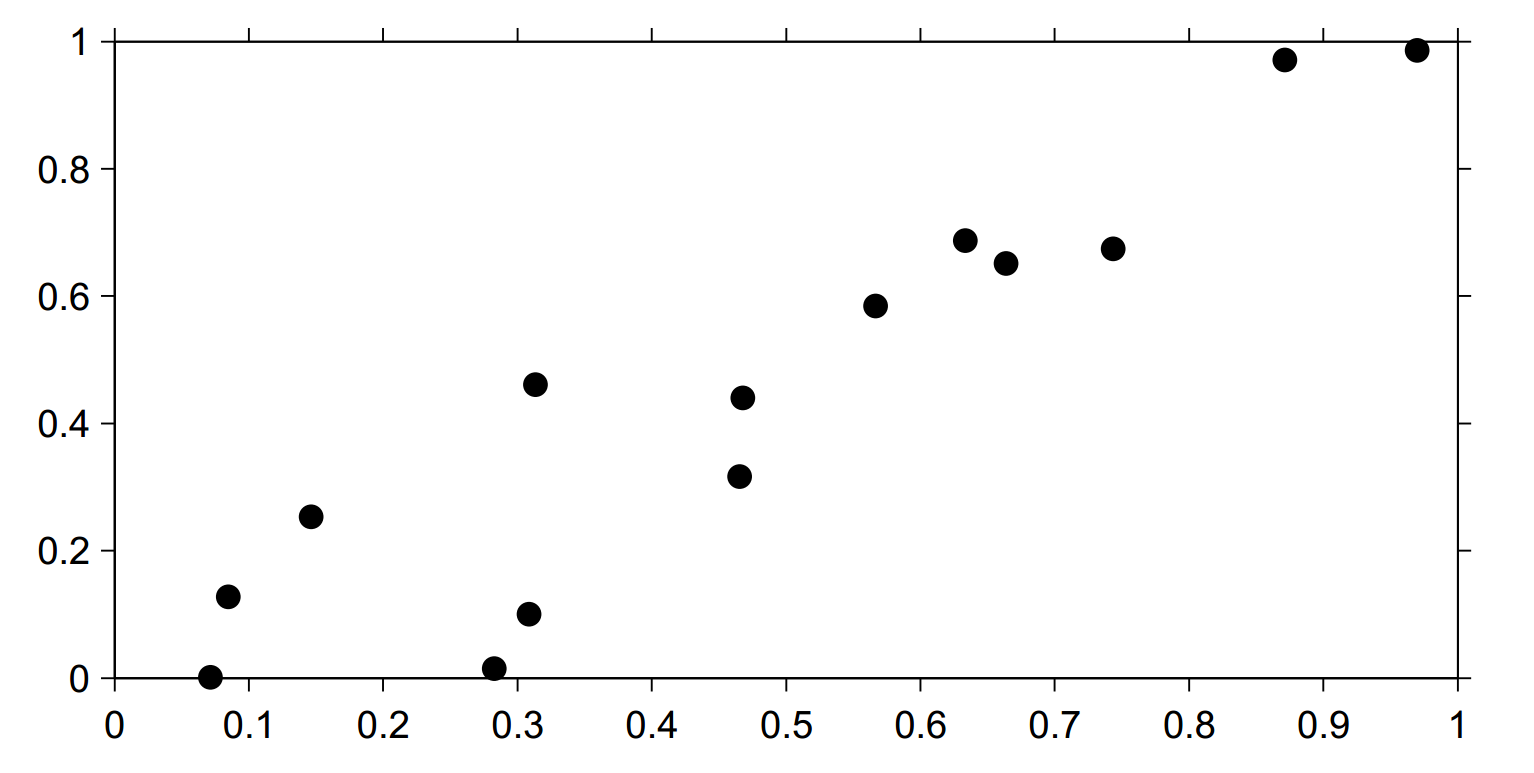
\includegraphics[scale=0.2]{Regression_1.png} 
\end{figure}
\textbf{Training data}: $\left\{(x_i, y_i) \colon i=\overline{1,N} \right\}$, $x_i, y_i \in R$

\textbf{Task}: given new $x^*$ predict $y^*$
\end{frame}

\begin{frame}{Three ways to go}
\begin{block}{Linear regression}
\end{block}
\begin{block}{Bayesian regression}
\end{block}
\begin{block}{Gaussian Process}
\end{block}
\end{frame}

\section{Linear regression}
\begin{frame}{Linear regression}
Utilize \textbf{model} 
$$
y = m x,
$$
\textbf{One should solve}
$$
m^* = arg\min_{m \in R} \sum_{i=1}^{N} (y_i - m  x_i)^2
$$
and get $m^*=\frac{\sum_ix_i y_i}{\sum_i x_i^2}$
\begin{figure}
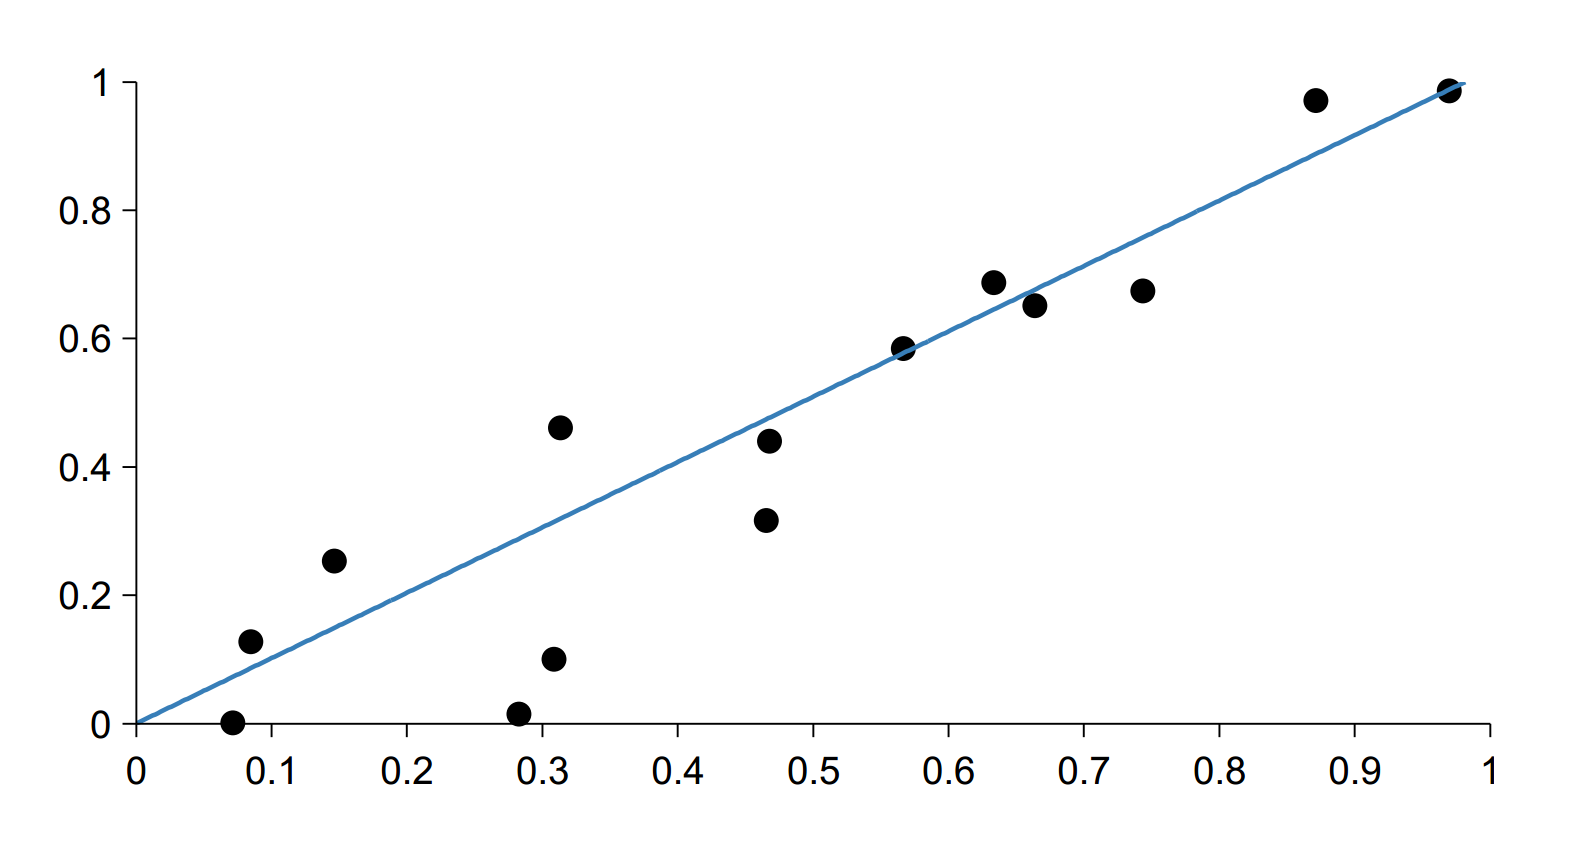
\includegraphics[scale=0.15]{Regression_2.png} 
\end{figure}
\end{frame}

\section{Bayesian regression}
\begin{frame}{Bayesian regression}
Utilize \textbf{model}
$$
y_i = m x_i + \varepsilon_i, \quad \varepsilon_i \sim_{\text{iid}} N(0,\sigma_{\varepsilon}^2), \quad m\sim N(0,1).
$$
\begin{figure}
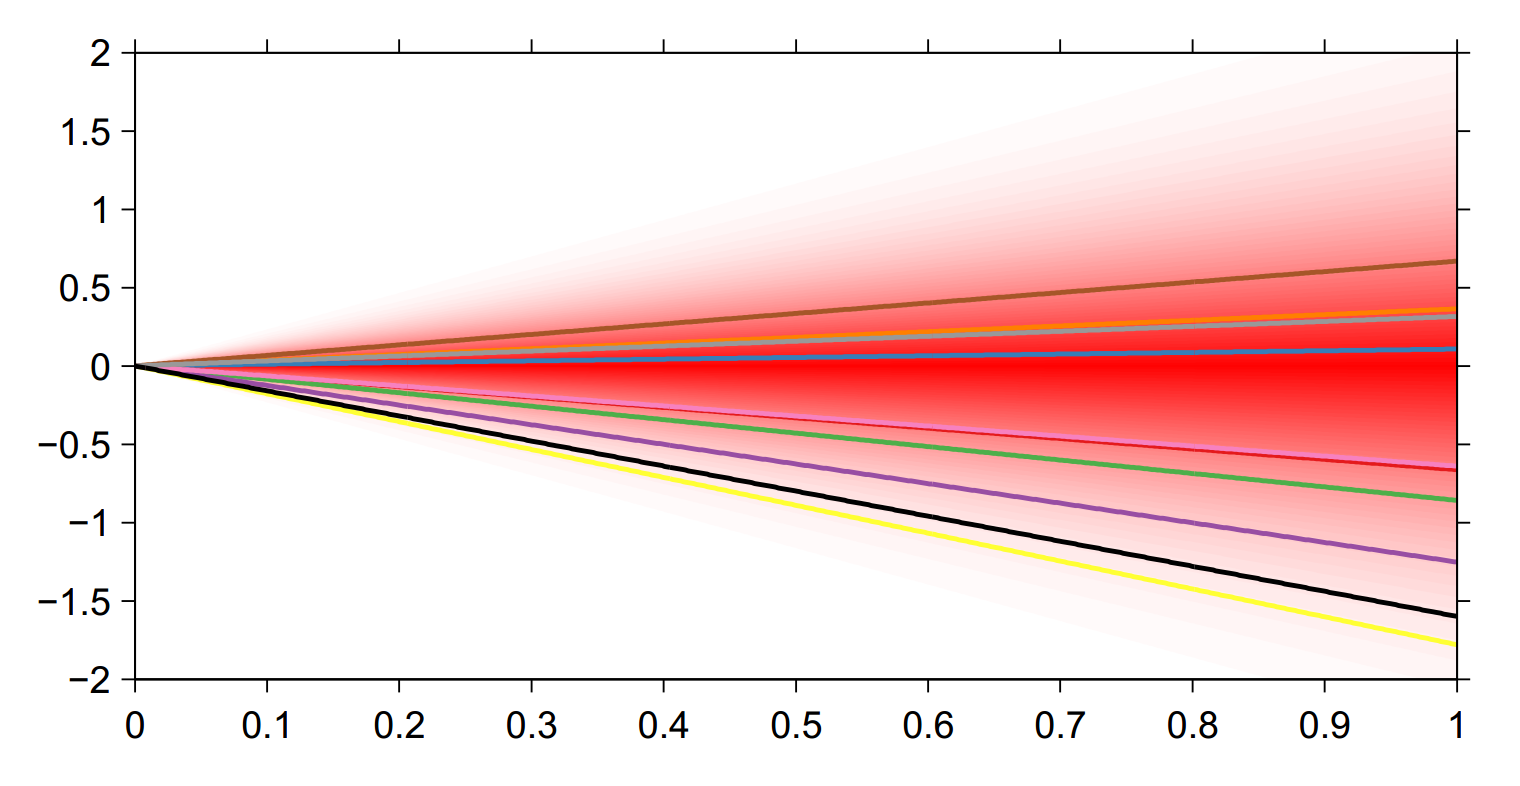
\includegraphics[scale=0.2]{Regression_3.png} 
\end{figure}
The goal is to find $p(m|y,x)$
\end{frame}


\begin{frame}{Bayesian formula}
\begin{align*}
    \onslide<1->{p(m|y,x) &= \frac{p(y|m,x) p(m)}{\int{p(y|m,x)p(m) dm}} \\} 
    \onslide<2->{&\propto p(y|m,x) p(m)\\ }
    \onslide<3->{&\propto\left(\prod_i \frac{1}{\sqrt{2\pi}\sigma_{\varepsilon}} e^{-(y_i-m x_i)^2/(2\sigma_{\varepsilon}^2)}\right) \frac{1}{\sqrt{2\pi}e^{-m^2/2}}\\} 
    \onslide<4->{&\propto e^{-\sum_i (y_i-m x_i)^2/(2\sigma_{\varepsilon}^2) - m^2/2} \\}
    \onslide<5->{&\propto e^{-\frac{\sum_i x_i^2 + \sigma_{\varepsilon}^2}{2\sigma_{\varepsilon}^2} \left(m-\frac{\sum_i x_i y_i}{\sum_i x_i^2 + \sigma_{\varepsilon}^2}\right)^2}}
\end{align*}
\onslide<6->{That is: {\color{red}$m|y,x \sim \mathcal{N}\left(\frac{\sum_i x_i y_i}{\sum_i x_i^2 + \sigma_{\varepsilon}^2},\frac{\sigma_{\varepsilon}^2}{\sum_i x_i^2 + \sigma_{\varepsilon}^2}\right)$}}
\end{frame}

\begin{frame}{Parameters posterior}
\begin{figure}
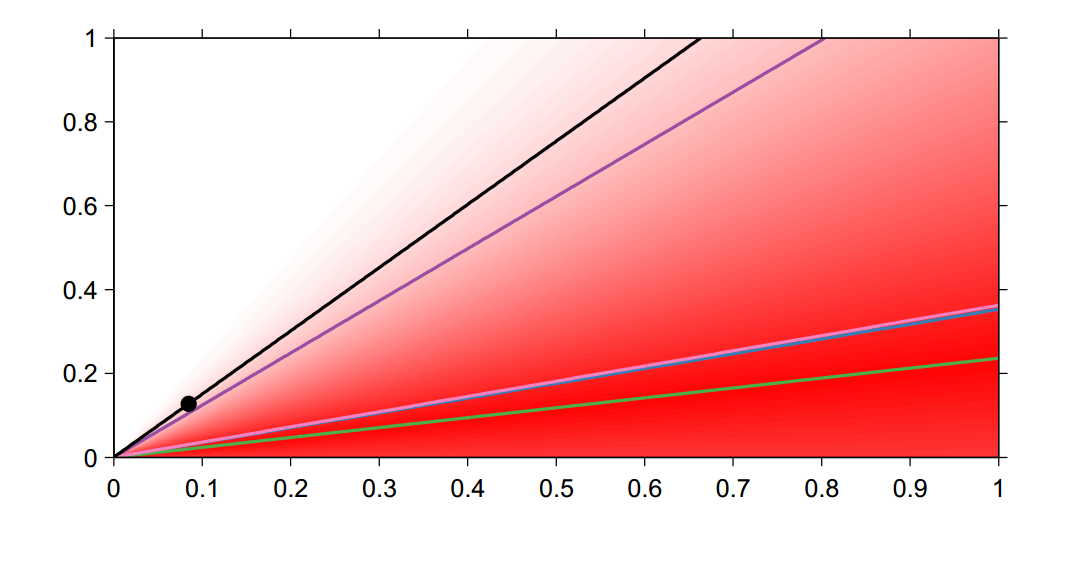
\includegraphics[scale=0.4]{Bayesian_1.png} 
\end{figure}
$$m|y,x \sim \mathcal{N}\left(\frac{\sum_i x_i y_i}{\sum_i x_i^2 + \sigma_{\varepsilon}^2},\frac{\sigma_{\varepsilon}^2}{\sum_i x_i^2 + \sigma_{\varepsilon}^2}\right)$$
\end{frame}


\begin{frame}{Parameters posterior}
\begin{figure}
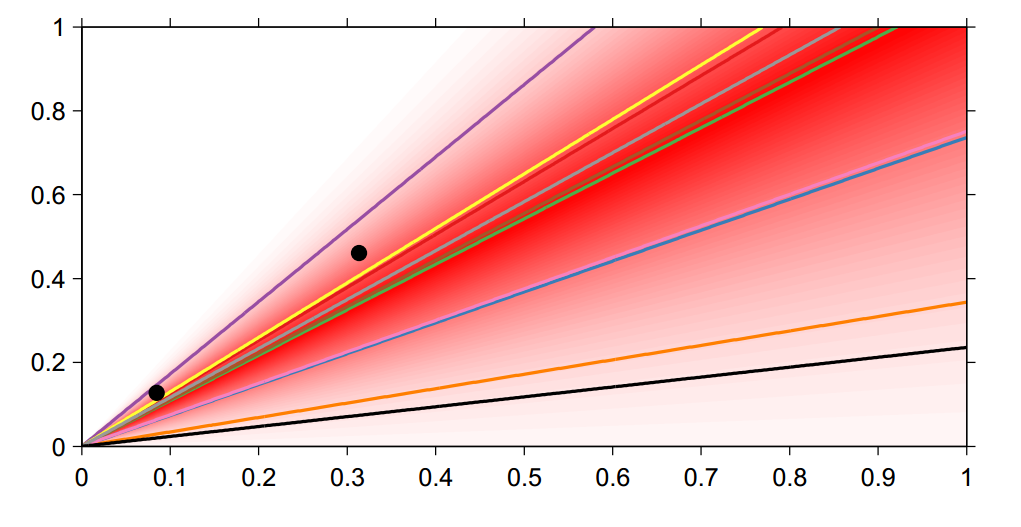
\includegraphics[scale=0.4]{Bayesian_2.png} 
\end{figure}
$$m|y,x \sim \mathcal{N}\left(\frac{\sum_i x_i y_i}{\sum_i x_i^2 + \sigma_{\varepsilon}^2},\frac{\sigma_{\varepsilon}^2}{\sum_i x_i^2 + \sigma_{\varepsilon}^2}\right)$$
\end{frame}

\begin{frame}{Parameters posterior}
\begin{figure}
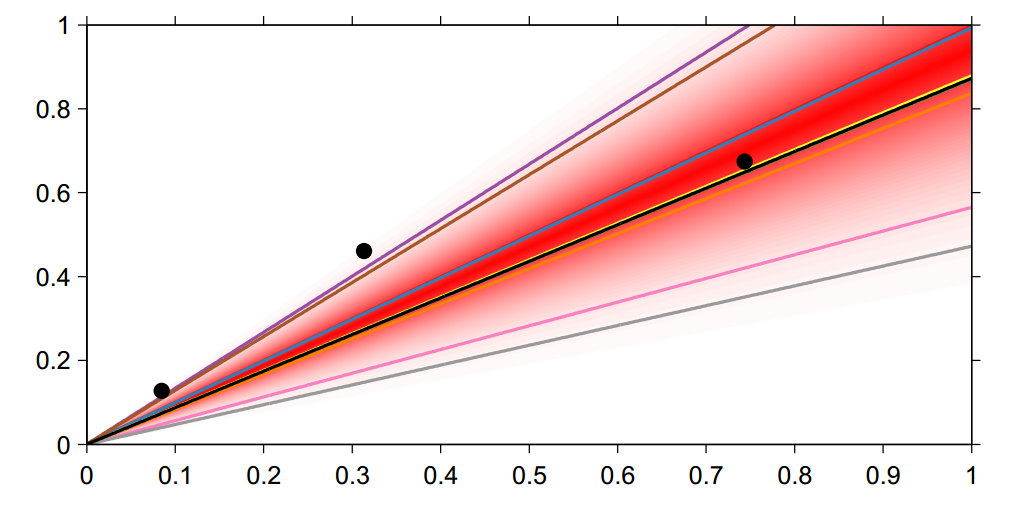
\includegraphics[scale=0.4]{Bayesian_3.png} 
\end{figure}
$$m|y,x \sim \mathcal{N}\left(\frac{\sum_i x_i y_i}{\sum_i x_i^2 + \sigma_{\varepsilon}^2},\frac{\sigma_{\varepsilon}^2}{\sum_i x_i^2 + \sigma_{\varepsilon}^2}\right)$$
\end{frame}

\begin{frame}{Parameters posterior}
\begin{figure}
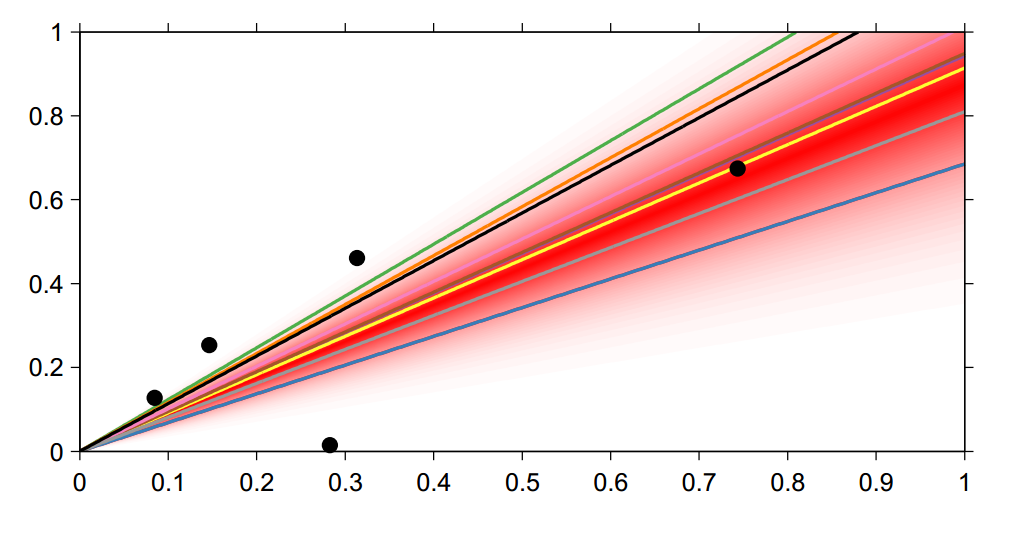
\includegraphics[scale=0.4]{Bayesian_4.png} 
\end{figure}
$$m|y,x \sim \mathcal{N}\left(\frac{\sum_i x_i y_i}{\sum_i x_i^2 + \sigma_{\varepsilon}^2},\frac{\sigma_{\varepsilon}^2}{\sum_i x_i^2 + \sigma_{\varepsilon}^2}\right)$$
\end{frame}

\begin{frame}{Parameters posterior}
\begin{figure}
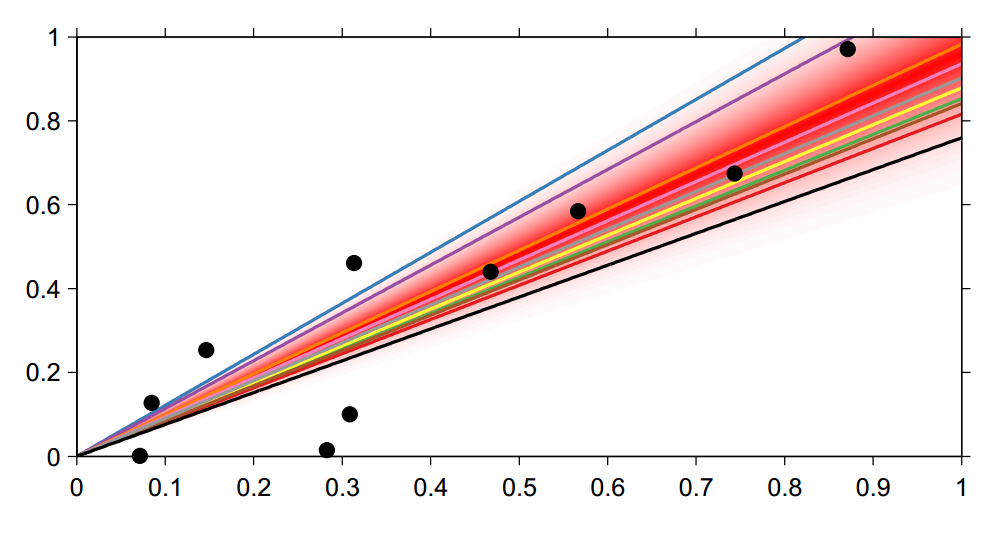
\includegraphics[scale=0.4]{Bayesian_5.png} 
\end{figure}
$$m|y,x \sim \mathcal{N}\left(\frac{\sum_i x_i y_i}{\sum_i x_i^2 + \sigma_{\varepsilon}^2},\frac{\sigma_{\varepsilon}^2}{\sum_i x_i^2 + \sigma_{\varepsilon}^2}\right)$$
\end{frame}

\begin{frame}{Parameters posterior}
\begin{figure}
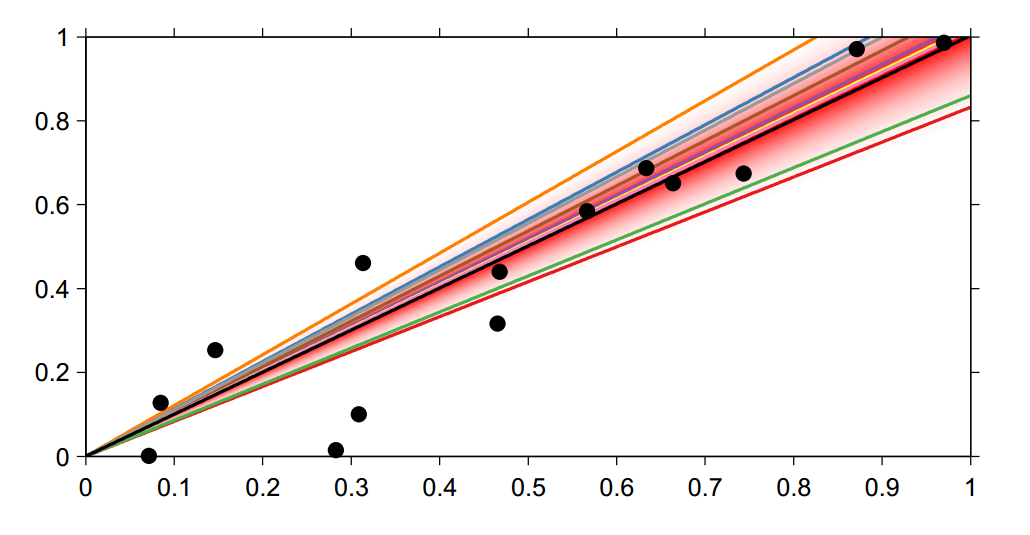
\includegraphics[scale=0.4]{Bayesian_6.png} 
\end{figure}
$$m|y,x \sim \mathcal{N}\left(\frac{\sum_i x_i y_i}{\sum_i x_i^2 + \sigma_{\varepsilon}^2},\frac{\sigma_{\varepsilon}^2}{\sum_i x_i^2 + \sigma_{\varepsilon}^2}\right)$$
\end{frame}

\begin{frame}{Output posterior}
\begin{align*}
    p(y^*|x^*,x,y)&=\int{p(y^*|x^*,m) p(m| x,y) dm} \\
    &= \mathcal{N}\left(x^* \frac{\sum_i x_i y_i}{\sum_i x_i^2 + \sigma_{\varepsilon}^2},(x^*)^2\frac{\sigma_{\varepsilon}^2}{\sum_i x_i^2 + \sigma_{\varepsilon}^2}\right)
\end{align*}
%Mean value {\color{red}$x^* \frac{\sum_i x_i y_i}{\sum_i x_i^2 + \sigma_{\varepsilon}^2}$} is exactly the least square solution. 
\pause

In more general case  $m \sim \mathcal{N}(\mathbf{0},\Sigma_p)$ and input space is multidimensional:
$$
y^*|x^*,x,y \sim \mathcal{N}\left(\frac{1}{\sigma_{\varepsilon}^2} \mathbf{x^*}^{\intercal} A^{-1} X \mathbf{y},\mathbf{x^*}^{\intercal} A^{-1}\mathbf{x^*})\right),
$$
where $A=\sigma_{\varepsilon}^{-2} X X^{\intercal} + \Sigma_p^{-1}$
\end{frame}

\begin{frame}{Input space to feature space}
Project input space with transformation $\phi(\mathbf{x})\colon \mathrm{R}^n \to \mathrm{R}^s$. $$\Phi= \Phi(X)=(\phi(\mathbf{x}_1),\phi(\mathbf{x}_2),\ldots, \phi(\mathbf{x}_N))$$
\pause
\textbf{Model} takes the form:
$$
\mathbf{y} = \phi(\mathbf{x})^{\intercal} \mathbf{m}
$$
\pause
\begin{multline*}
y^*|x^*,x,y \sim \mathcal{N}\left( {\phi^*}^{\intercal} \Sigma_p\Phi^{-1} (K+\sigma_{\varepsilon}^2 I)^{-1} \mathbf{y},\right.\\
\left.{\phi^*}^{\intercal} \Sigma_p {\phi^*} - {\phi^*}^{\intercal} \Sigma_p\Phi (K+\sigma_{\varepsilon}^2 I)^{-1} \Phi^{\intercal} \Sigma_p\phi^* \right),
\end{multline*}
\pause
where ${\phi^*} = \phi(\mathbf{x^*})$ and $K=\Phi^{\intercal}\Sigma_p\Phi$
\end{frame}


\begin{frame}{From Bayesian regression to GP }
\begin{itemize}
    \item We defined a Bayesian linear regression model by specifying priors on $m$ and $\varepsilon_i$\pause
    \begin{itemize}
        \item $m\sim \mathcal{N}$, $\varepsilon_i \sim_{\text{iid}} \mathcal{N}(0, \sigma_{\varepsilon}^2)$\pause
        \item $y_i|m,\varepsilon_i = m x_i + \varepsilon_i$\pause
    \end{itemize}
    \item This implicitly defined a joint prior on $\{y_i\colon i=\overline{1,n}\}$ \pause
    \begin{itemize}
        \item $y_i\sim \mathcal{N}(0,x_i^2 + \sigma_{\varepsilon}^2)$\pause
        \item $cov(y_i,y_j) = x_i x_j$, $\forall i\neq j$
    \end{itemize}
\end{itemize}
\pause
That is $(y_1, y_2, \ldots, y_n)$ has multivariate normal distribution:
$$
y\sim \mathcal{N}(\textbf{0},\textbf{K}), \quad k_{ij}=x_i x_j + \delta_{ij}\sigma_{\varepsilon}^2
$$
\end{frame}






\begin{frame}{Gaussian processes}
    \begin{block}{Definition}
    Gaussian process is a collection of random variables, any finite number of which have a joint Gaussian distribution 
    \end{block}\pause
    We can write this collection of random variables as
    $$
    \left\{f(x)\colon x\in \mathcal{X} \right\}
    $$
    i.e. a function $f$ evaluated at inputs $x$.
    \pause
    \begin{block}{GP($\mu$,$k$) is completely specified by}\pause
    \begin{itemize}
        \item Mean function $\mu(x)=\mathrm{E}(f(x))$\pause
        \item Covariance/kernel function $k(x,x') = Cov(f(x),f(x'))$
    \end{itemize}
    \end{block}
\end{frame}


\begin{frame}{Linear kernel}
\begin{figure}
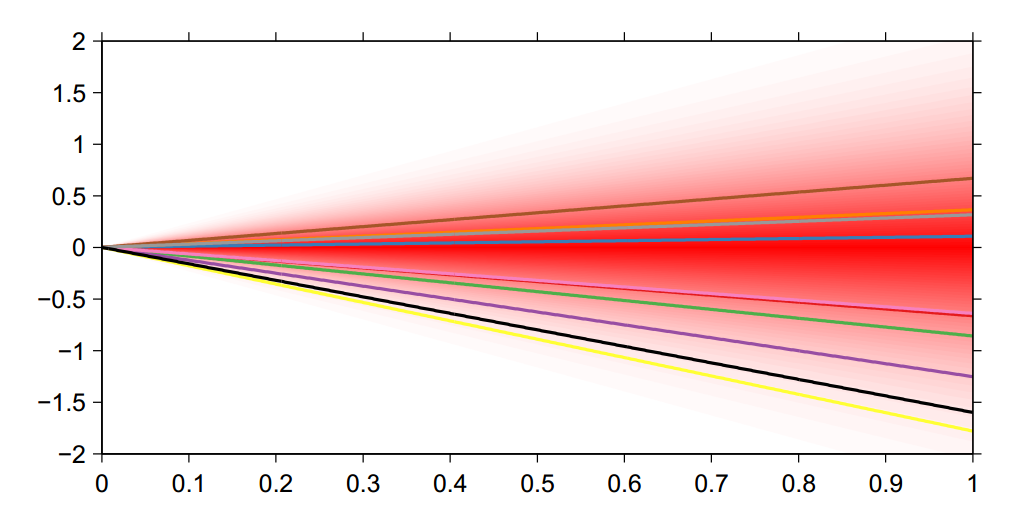
\includegraphics[scale=0.4]{Bayesian_non_linear_1.png} 
\end{figure}
$$
k(x,x')=x x'
$$
\end{frame}

\begin{frame}{Exponential kernel}
\begin{figure}
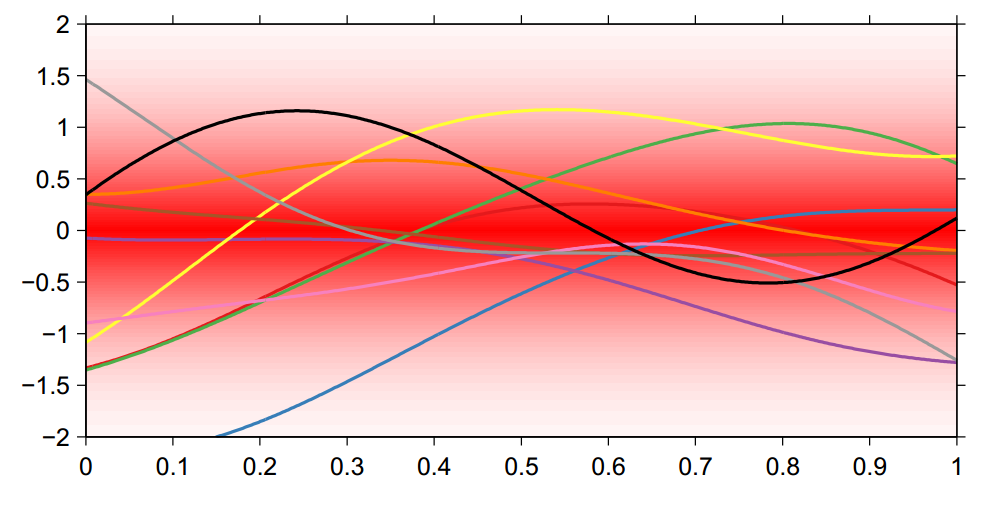
\includegraphics[scale=0.4]{Bayesian_non_linear_2.png} 
\end{figure}
$$
k(x,x')=e^{-(x-x')^2}
$$
\end{frame}
\begin{frame}{Non-linear kernel}
\begin{figure}
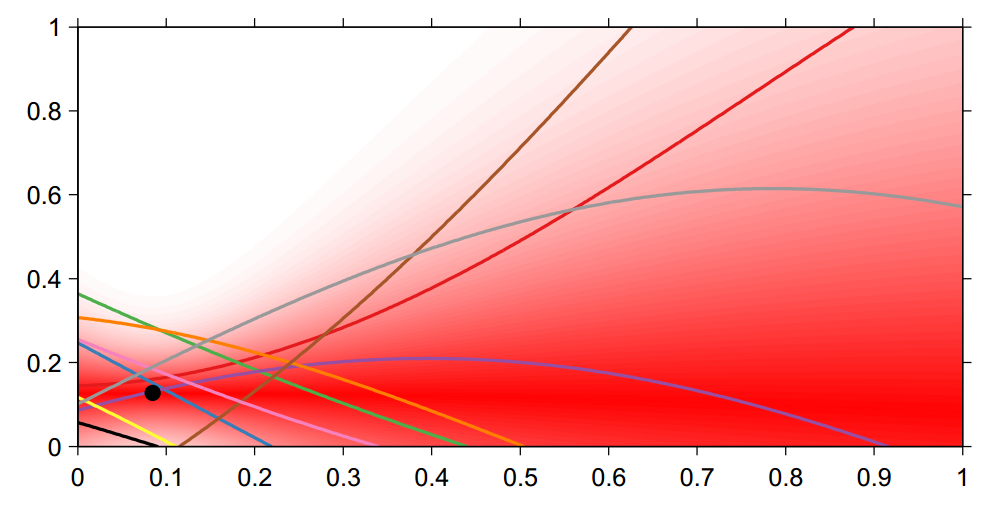
\includegraphics[scale=0.4]{Bayesian_non_linear_3.png} 
\end{figure}
\end{frame}
\begin{frame}{Non-linear kernel}
\begin{figure}
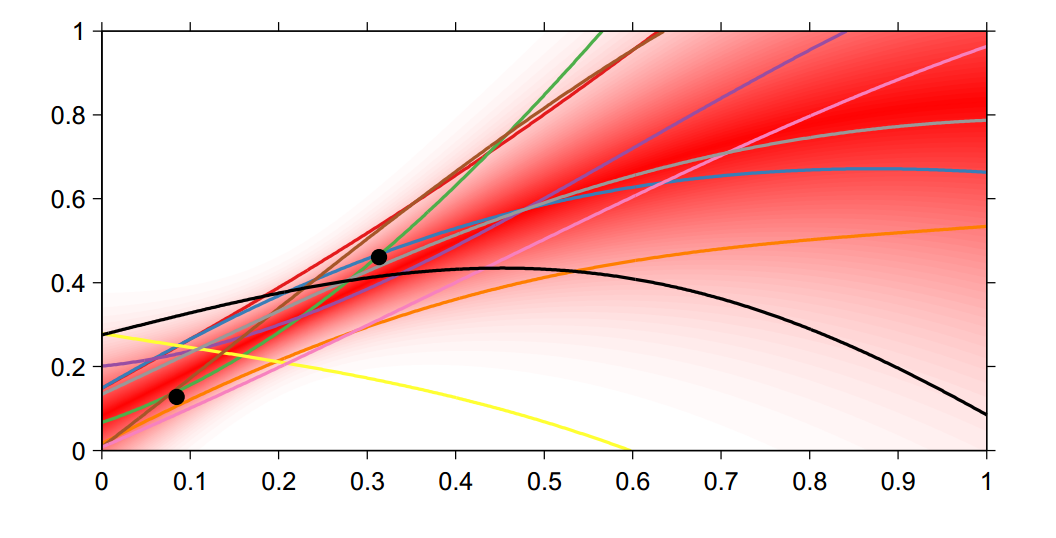
\includegraphics[scale=0.4]{Bayesian_non_linear_4.png} 
\end{figure}
\end{frame}
\begin{frame}{Non-linear kernel}
\begin{figure}
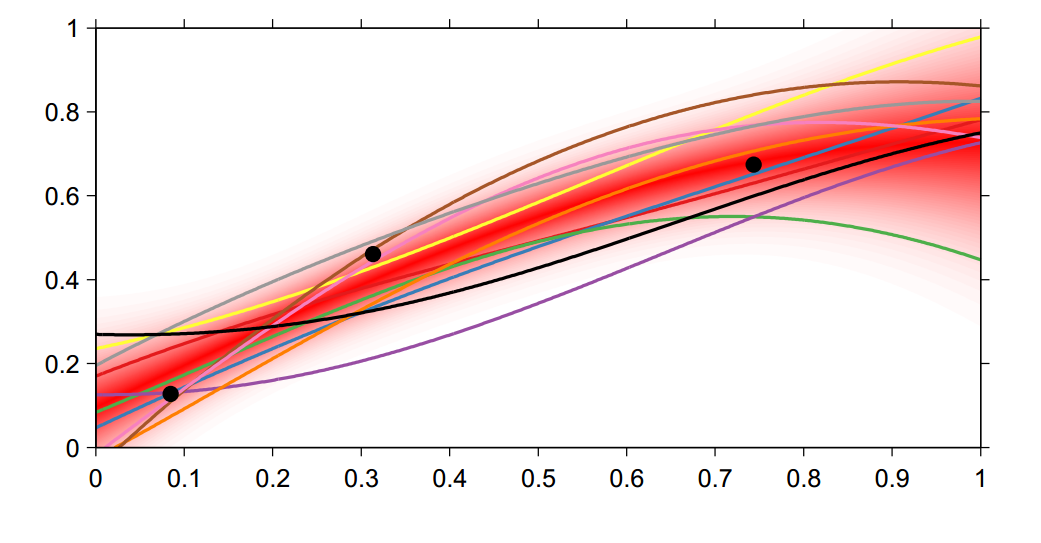
\includegraphics[scale=0.4]{Bayesian_non_linear_5.png} 
\end{figure}
\end{frame}
\begin{frame}{Non-linear kernel}
\begin{figure}
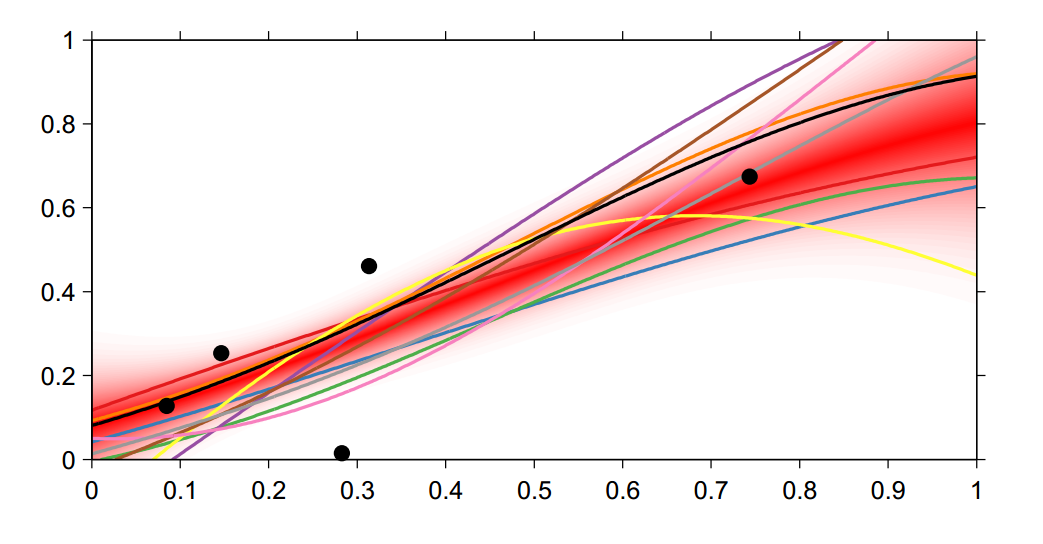
\includegraphics[scale=0.4]{Bayesian_non_linear_6.png} 
\end{figure}
\end{frame}
\begin{frame}{Non-linear kernel}
\begin{figure}
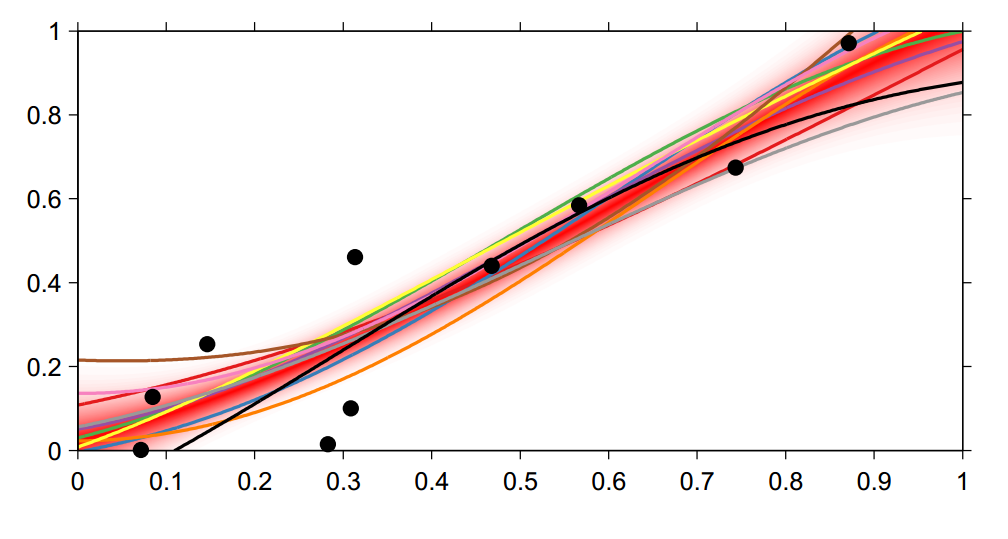
\includegraphics[scale=0.4]{Bayesian_non_linear_7.png} 
\end{figure}
\end{frame}
\begin{frame}{Non-linear kernel}
\begin{figure}
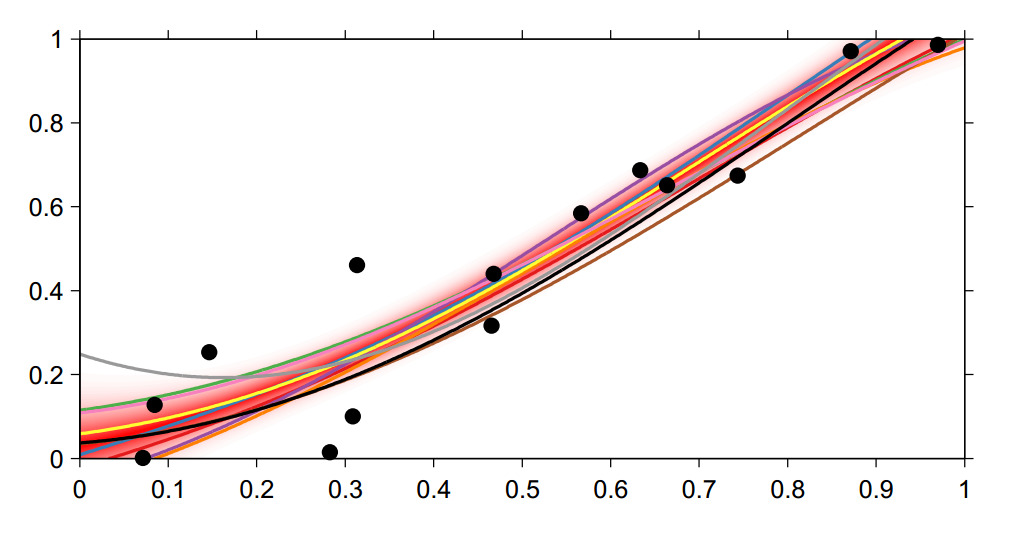
\includegraphics[scale=0.4]{Bayesian_non_linear_8.png} 
\end{figure}
\end{frame}
\begin{frame}{Linear model gone wrong}
\begin{figure}
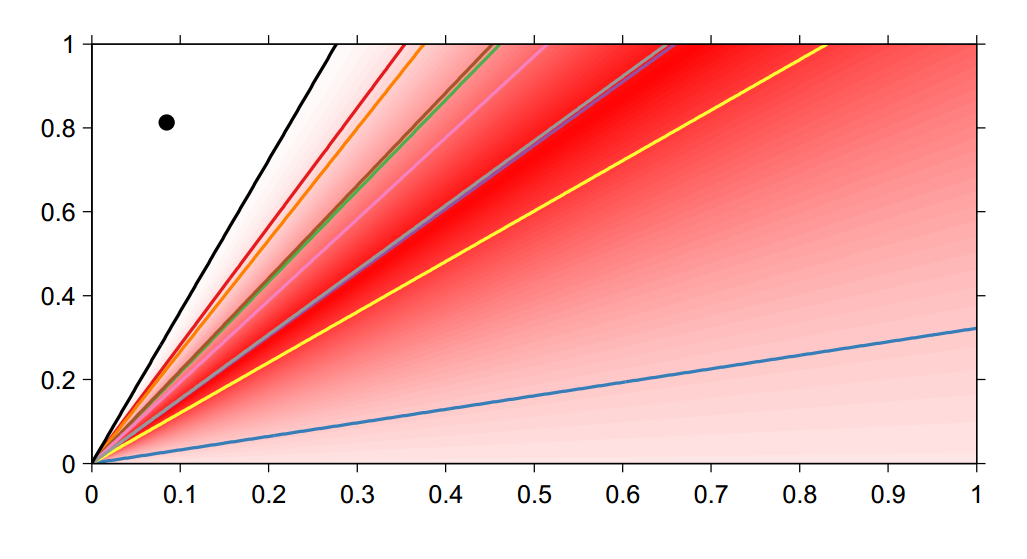
\includegraphics[scale=0.4]{Bayesian_non_linear_9.png} 
\end{figure}
\end{frame}
\begin{frame}{Linear model gone wrong}
\begin{figure}
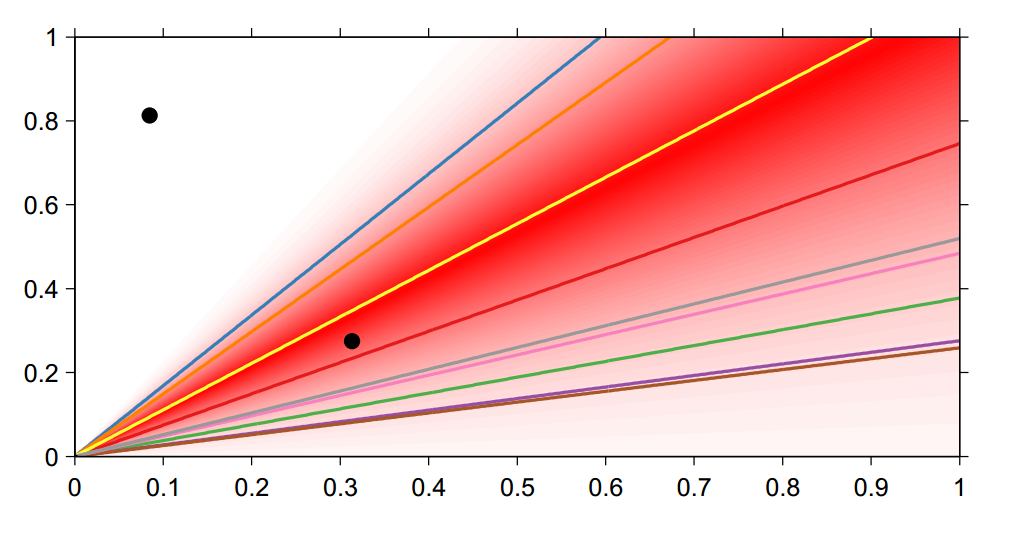
\includegraphics[scale=0.4]{Bayesian_non_linear_10.png} 
\end{figure}
\end{frame}
\begin{frame}{Linear model gone wrong}
\begin{figure}
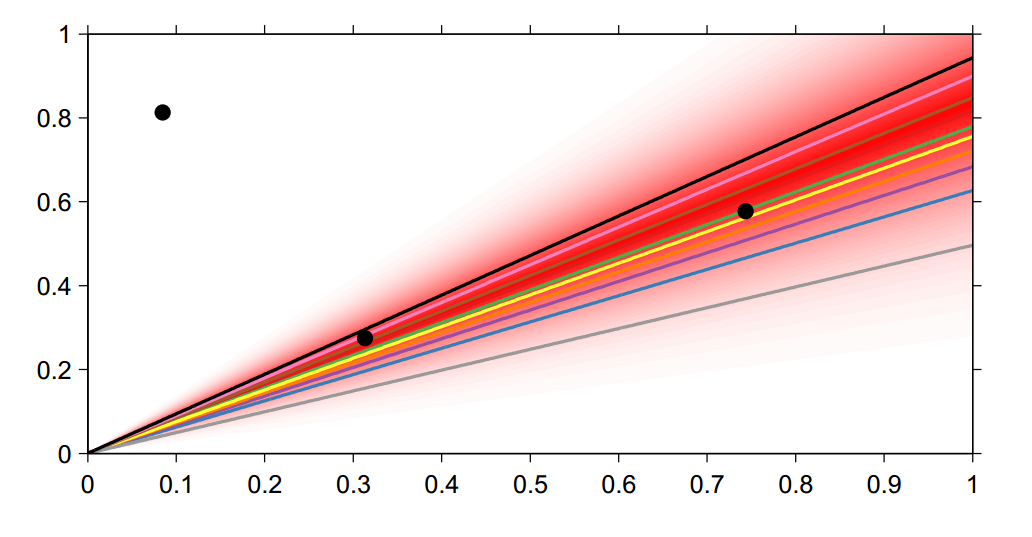
\includegraphics[scale=0.4]{Bayesian_non_linear_11.png} 
\end{figure}
\end{frame}
\begin{frame}{Linear model gone wrong}
\begin{figure}
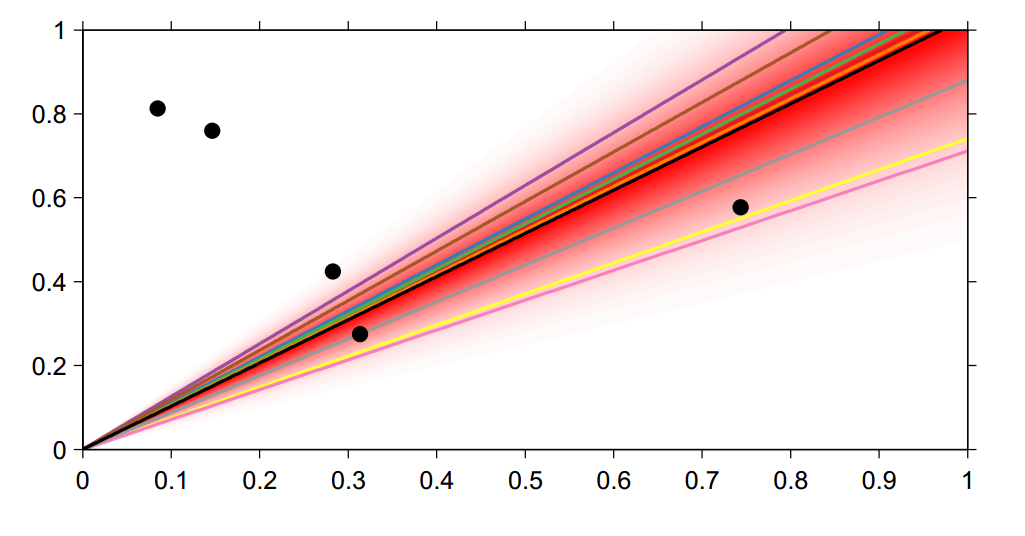
\includegraphics[scale=0.4]{Bayesian_non_linear_12.png} 
\end{figure}
\end{frame}
\begin{frame}{Linear model gone wrong}
\begin{figure}
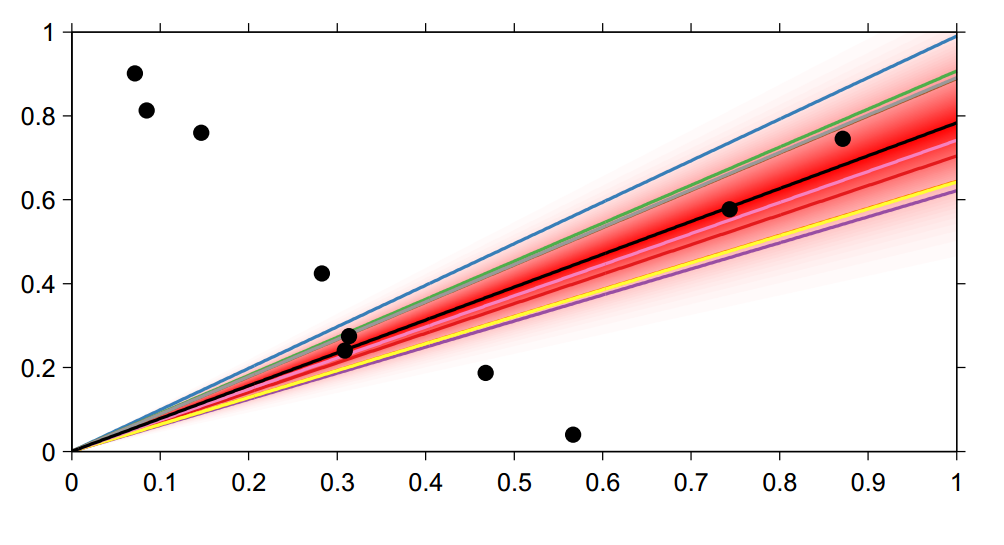
\includegraphics[scale=0.4]{Bayesian_non_linear_13.png} 
\end{figure}
\end{frame}

\begin{frame}{Linear model gone wrong}
\begin{figure}
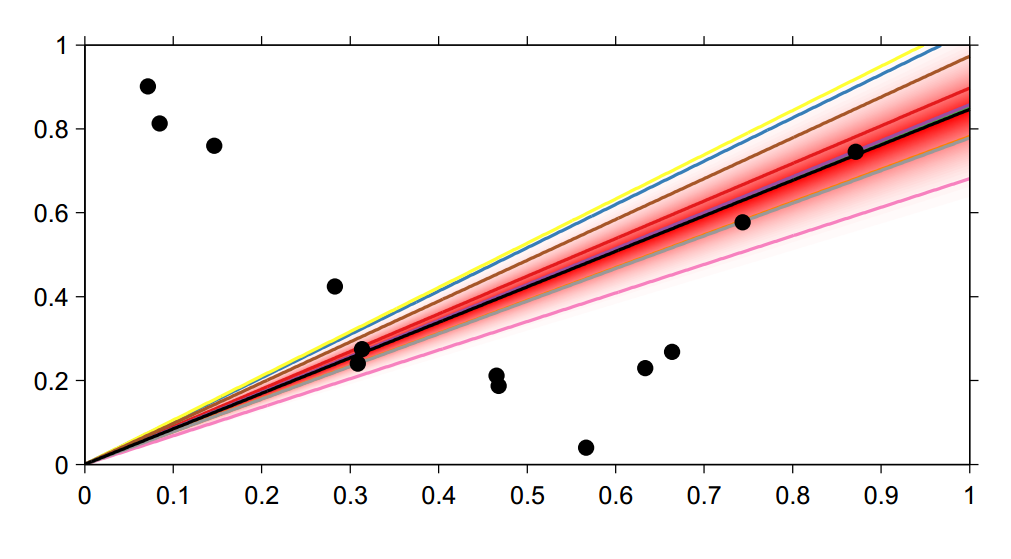
\includegraphics[scale=0.4]{Bayesian_non_linear_14.png} 
\end{figure}
\end{frame}

\begin{frame}{Non-linearity to the rescue}
\begin{figure}
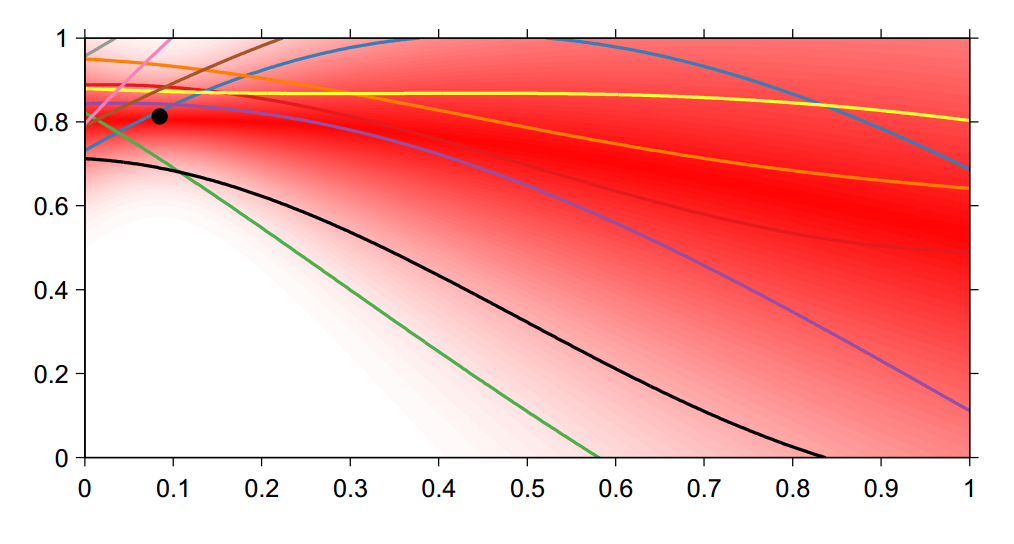
\includegraphics[scale=0.4]{Bayesian_non_linear_15.png} 
\end{figure}
\end{frame}

\begin{frame}{Non-linearity to the rescue}
\begin{figure}
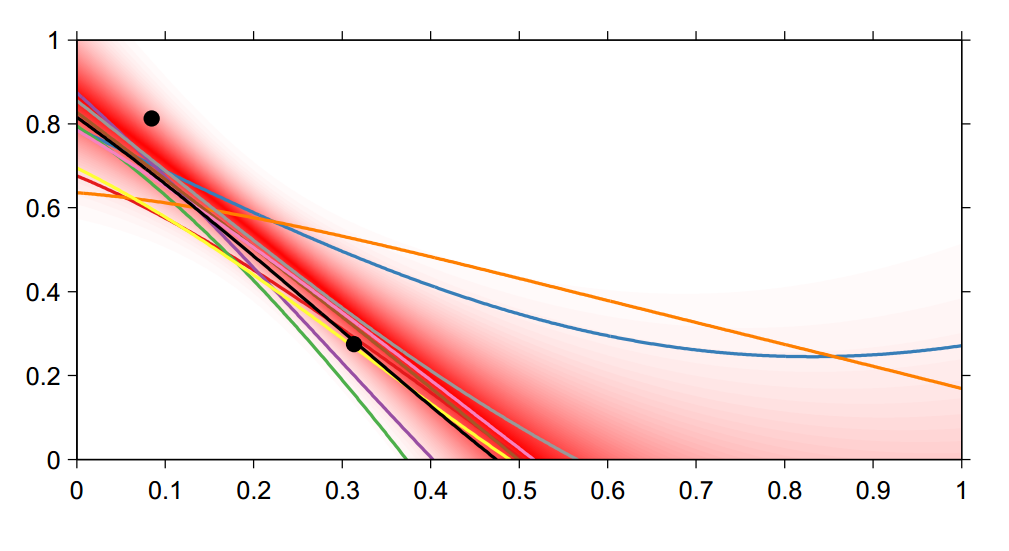
\includegraphics[scale=0.4]{Bayesian_non_linear_16.png} 
\end{figure}
\end{frame}

\begin{frame}{Non-linearity to the rescue}
\begin{figure}
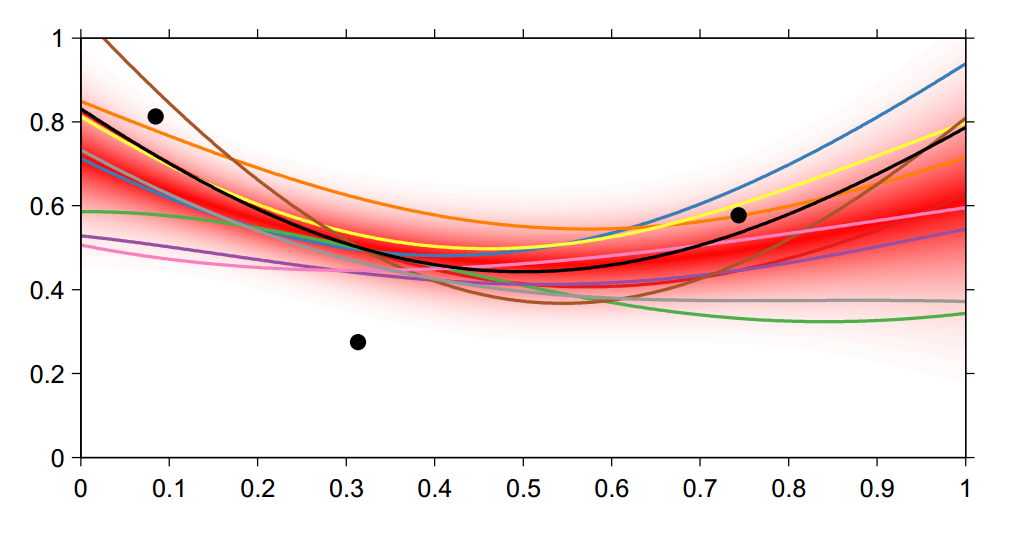
\includegraphics[scale=0.4]{Bayesian_non_linear_17.png} 
\end{figure}
\end{frame}
\begin{frame}{Non-linearity to the rescue}
\begin{figure}
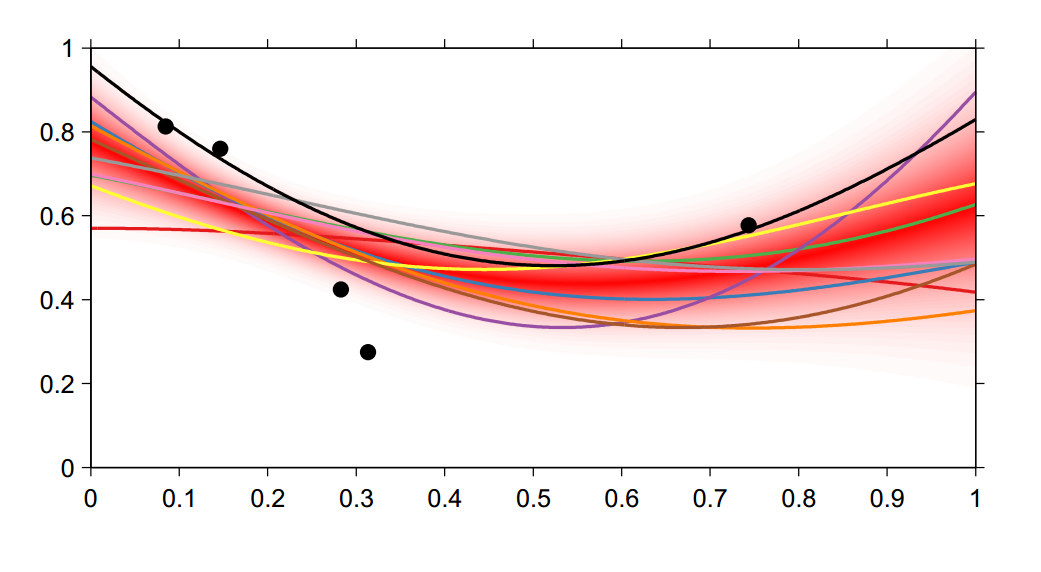
\includegraphics[scale=0.4]{Bayesian_non_linear_18.png} 
\end{figure}
\end{frame}
\begin{frame}{Non-linearity to the rescue}
\begin{figure}
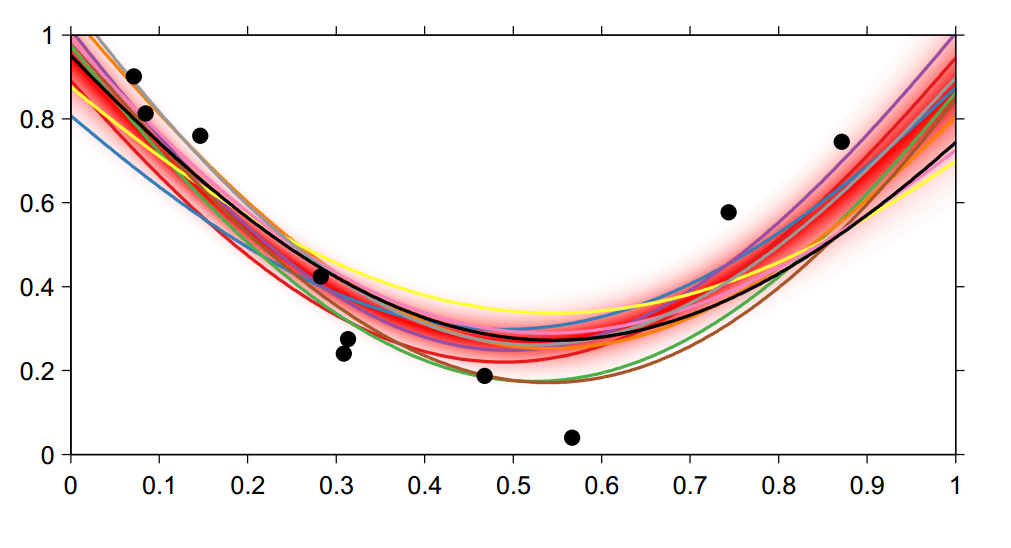
\includegraphics[scale=0.4]{Bayesian_non_linear_19.png} 
\end{figure}

\end{frame}
\begin{frame}{Non-linearity to the rescue}
\begin{figure}
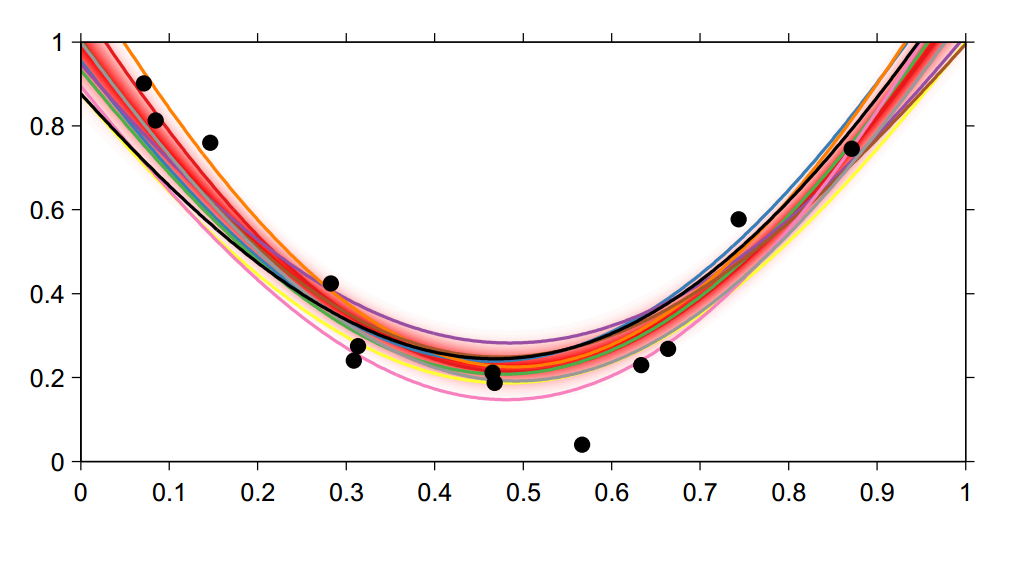
\includegraphics[scale=0.4]{Bayesian_non_linear_20.png} 
\end{figure}
\end{frame}

\begin{frame}{Kernel types}
\begin{figure}
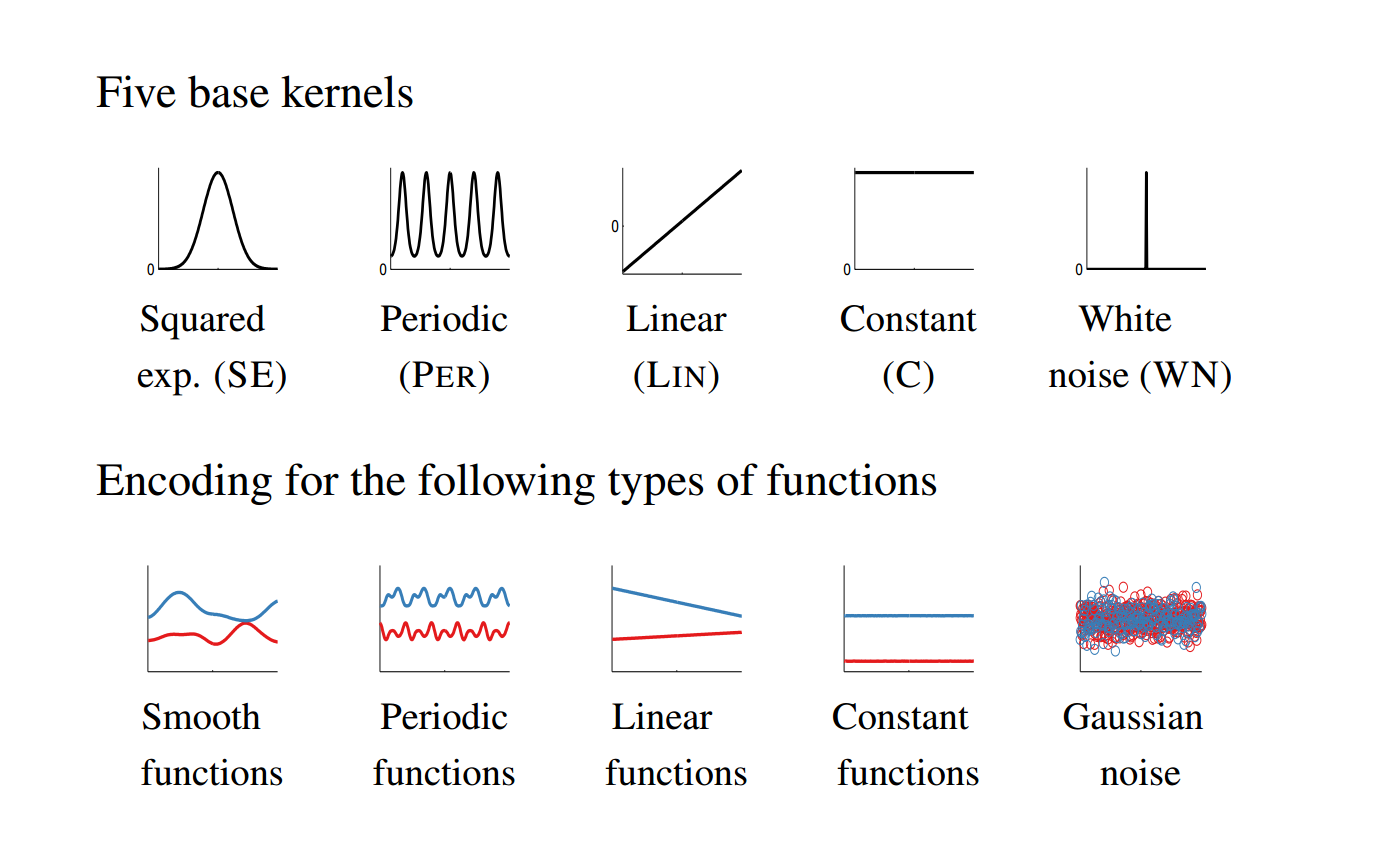
\includegraphics[scale=0.3]{Kernels_list.png} 
\end{figure}
\end{frame}

\begin{frame}{Kernels compositions}
\begin{figure}
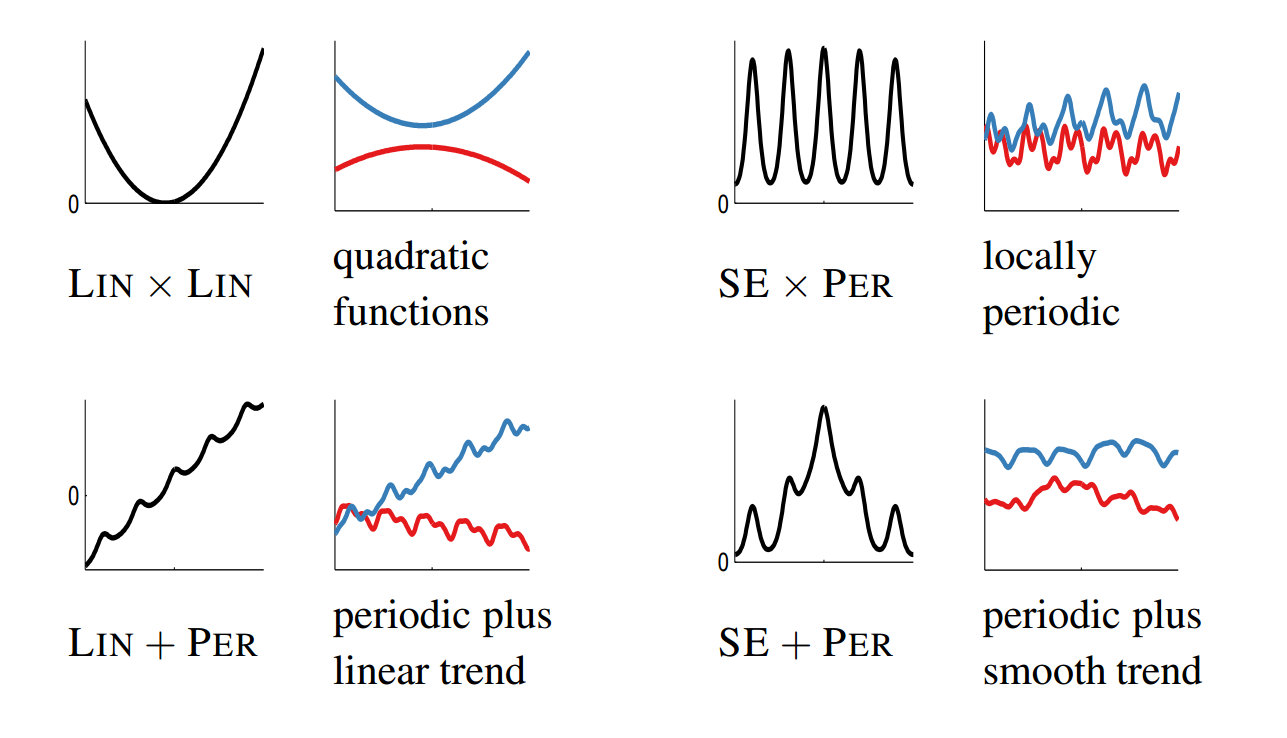
\includegraphics[scale=0.3]{Kernels_composition.png} 
\end{figure}
\end{frame}

\begin{frame}{Classification problem}
\textbf{Training data}: $\left\{(\mathbf{x}_i, y_i) \colon i=\overline{1,N} \right\}$, $\mathbf{x}_i \in R^s$, $y_i \in C=\{-1, +1\}$.

\textbf{Task}: given new $x^*$ predict distribution $y^*$ on $C$. 

That is we want to know 
$$
\pi(x)=p(y=+1 | \mathbf{x}).
$$
\end{frame}

\begin{frame}{Classification problem solving}
\textbf{Main idea:} 
$$\pi(x)= \sigma(f(\mathbf{x})),$$
$f(\cdot)$ --- latent variable.
\begin{block}{Step 1}
$$p(f^* |X,y,\mathbf{x}^*) = \int{p(f^* |X,\mathbf{x}^*,\mathbf{f})p(\mathbf{f}|X,y)df}$$
\end{block}
\begin{block}{Step 2}
$$p(y^*=+1 |X,y,\mathbf{x}^*) = \int{\sigma(f^*) p(f^*|X,y,\mathbf{x}^*)df^*}$$
\end{block}

\end{frame}

\end{document}
